\documentclass[11pt,a4paper]{article} % Font size and paper type
\pagestyle{empty} % Suppress page numbers
\usepackage[left=1.9cm,top=2cm,right=2cm,bottom=1cm]{geometry}
\usepackage[utf8]{inputenc}
\usepackage[dvipsnames]{xcolor}
\usepackage[parfill]{parskip} % Remove paragraph indentation
\usepackage{graphicx}
\usepackage{enumitem}
\setitemize{itemsep=-5pt,leftmargin=*,label={-},topsep=-5pt}
\usepackage[colorlinks=true,urlcolor=MidnightBlue]{hyperref}

\newcommand{\hSection}[1]{
    \medskip
    \MakeUppercase{\bf #1}
    \medskip
    \hrule
}
\newcommand{\hSubsectionI}[2]{{\bf #1}\hfill {#2}\hspace{-1cm}}
\newcommand{\hSubsection}[2]{{\bf #1}\hfill {#2}}

\begin{document}

\begin{center}
    {\LARGE \bf VILÉM ZOUHAR} \\
    {\large \href{mailto:vilem.zouhar@gmail.com}{\color{black}{vilem.zouhar@gmail.com}}}
\end{center}

\vspace{0.1cm}

\begin{minipage}{0.75\textwidth}
\hSection{Education}\vspace{0.2cm}
{\bf Charles University in Prague} \hfill {2017/18 - 2019/20} \\
BSc. in Computer Science \\
specialization in Computational linguistics \\
Thesis \href{https://dspace.cuni.cz/bitstream/handle/20.500.11956/119400/130284419.pdf?sequence=1&isAllowed=y}{Enabling Outbound Machine Translation}


{\bf Saarland University + Groningen University} \hfill {2020/21 - exp. 2022/23} \\
MSc. in Language Science and Technology \\
Double degree programme
\end{minipage}
% 
% 
\begin{minipage}{0.25\textwidth}
  \vspace{-2cm}
  \hfill
  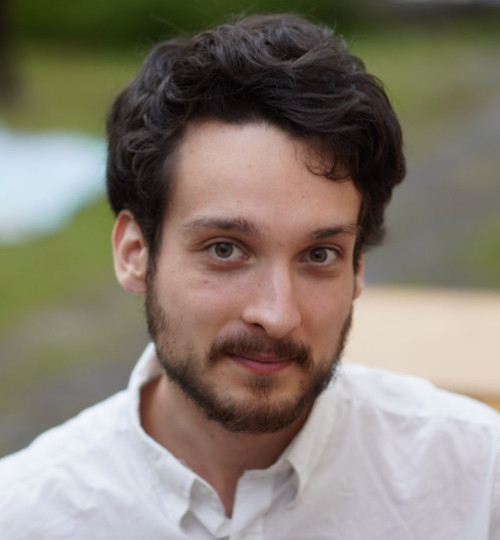
\includegraphics[width=3.5cm]{portrait.jpg}
  \vspace{-0.9cm}
\end{minipage}

\hSection{Academic Projects and Publications}

\hSubsectionI{Outbound Translation User Interface Ptakopet: A Pilot Study}{\href{https://www.aclweb.org/anthology/2020.lrec-1.860.pdf}{LREC 2020} published}

\hSubsectionI{Extending Ptakopět for MT User Interaction Experiments}{\href{https://ufal.mff.cuni.cz/pbml/115/art-zouhar-novak.pdf}{PBML 115} published}

\hSubsectionI{WMT20 Document-Level Markable Error Exploration}{to be published in WMT20}

\hSubsectionI{Paper on machine translation application}{in an anonymized review process}

\hSubsectionI{Paper on machine translation evaluation}{in writing}

\hSubsectionI{A Collection of Machine Learning Excercises}{2018/2019}

\begin{itemize}
    \item 50 pages of ML tasks with solutions in R
    \item Full version with solutions available only per request (used as \href{http://ufal.mff.cuni.cz/courses/npfl054}{teaching material})
\end{itemize}
% hsection override
% {\bf Lost in Back-Translation:}\hfill{planned in Spring 2020} \\
% {\bf Which Translation Errors Get Recovered by Reverse MT System?}
% \begin{itemize}
%     \item Spin-off of our backtranslation research
% \end{itemize}

\begin{minipage}{.55\textwidth}
    \hSection{Technical Knowledge}
    \hspace{-0.3cm}
    \begin{minipage}{\textwidth}
        \vspace{0.15cm}
        \begin{tabular}{ l l}
        {\bf Programming} & JS/TS, Rust, C/C++, Python, R \\
        {\bf Toolkits} & TensorFlow 2.0+, NLTK \\
        {\bf Misc.} & Bash, UNIX/Linux proficiency \\
        \cr
        \end{tabular}
    \end{minipage}
\end{minipage}
\begin{minipage}{.45\textwidth}
    \hSection{Language Proficiency}
    \hspace{-0.3cm}
    \begin{minipage}{\textwidth}
        \vspace{0.15cm}
        \begin{tabular}{ l l}
        {\bf Czech} & Native \\
        {\bf English} & C1-C2\\
        {\bf German} & B1-B2 \textit{(in development)} \\
        {\bf Polish} & A1-A2
        \end{tabular}
    \end{minipage}
\end{minipage}

\vspace{-0.5cm}
\hSection{Work Experience}
\hSubsection{Institute of Formal and Applied Linguistics (student research assistant)}{2018-present} \\
\textbf{Charles Univeristy Faculty of Mathematics and Physics in Prague}\\
Participation in the \href{https://browser.mt/}{Bergamot project} and other miscellaneous research tasks

\hSubsection{Previo (intern software dev)}{summer 2018} \\
Development of multilayer CMS using JS, PHP, Zend and MySQL

\hSubsection{BIM Project (intern software dev)}{summer 2017} \\
Development of plugins for the ArchiCAD suite with C++/Boost and C\#

\hSubsection{Web development}{2015-2017} \\
Participation in several commercial projects: Brno bez vizuálního smogu, MrFox,\\Velab, Intimedcare using the PHP/JS/HTML/CSS stack

\hSection{Extra-Curricular}
\hSubsection{Academic senate}{2018-2020} \\
Member of the Academic Senate at Charles University Faculty of Mathematics and Physics

\hSubsection{Game Jams}{2015-2020} \\
Various game jams, mostly Ludum Dare; several \href{https://github.com/allemansratten}{games} programmed and presented in limited time

\hSubsection{Misc. projects}{present} \\
Small projects either for convenience, or as a hobby; code hosted at \href{https://github.com/zouharvi}{GitHub}

\hSubsection{Kasiopea}{2017-2019} \\
Organization of Kasiopea, an annual coding competition for highschool students

\end{document}

